%-------------------------------------------------------------------------------
% Section - Methodology (first version)
% Notation matches figures/methodology_scheme.svg
%-------------------------------------------------------------------------------
\section{Hybrid BEM--PINN Inversion}\label{sec:methodology}

The inversion strategy extends the BEM--PINN formulation of \citet{wu_novel_2026}
from forward scattering to geometric and material identification. A neural
network represents the source densities of an indirect boundary element
formulation, so the governing equation and the radiation condition are satisfied
exactly by construction, while the boundary conditions and the seismic records
enter as penalties in a single loss function. The geometric and material
unknowns are treated as additional trainable variables and are updated jointly
with the network weights (Fig.~\ref{fig:methodology_scheme}).

\begin{figure*}[ht!]
    \centering
    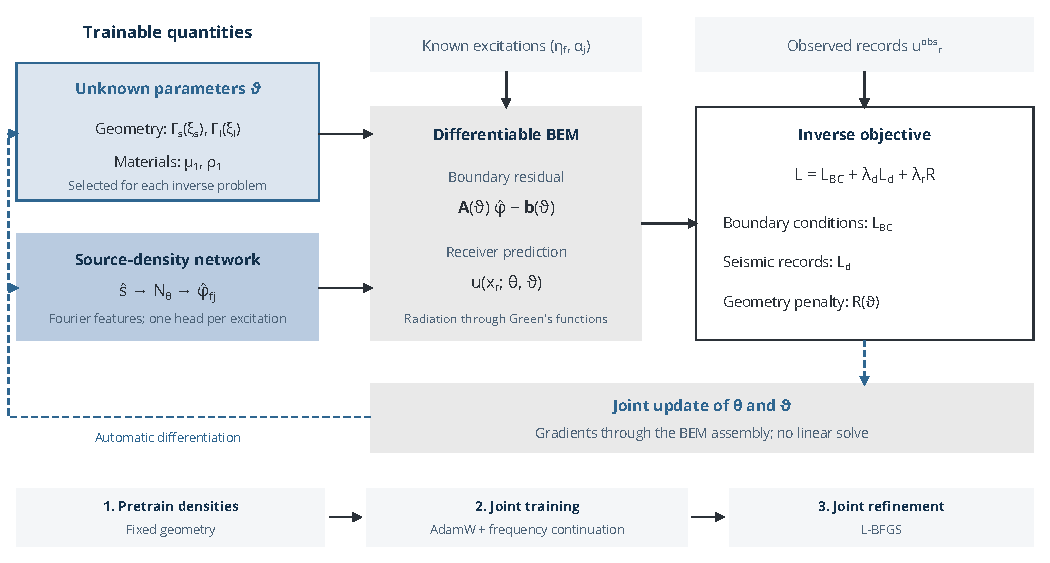
\includegraphics[width=6.5in]{figures/methodology_scheme.pdf}
    \caption{Inverse-oriented BEM--PINN workflow. The selected geometric and
      material unknowns $\vartheta$ and the network densities feed the
      differentiable BEM, which evaluates boundary residuals and receiver
      responses. A single objective combines boundary consistency, agreement
      with seismic records and geometric regularization. Dashed blue arrows
      show the joint update of $\vartheta$ and the network weights $\theta$
      by automatic differentiation, without a linear solve. The network uses
      Fourier features of $\hat s$ and one output head per excitation
      $(\eta_f,\alpha_j)$; the lower strip summarizes the training stages.}
    \label{fig:methodology_scheme}
\end{figure*}

\subsection{Forward model}

We consider antiplane (SH) motion with time dependence $e^{i\omega t}$. The
irregularity $\Omega_1$, with shear modulus $\mu_1$ and density $\rho_1$, is
bounded by the free surface $\Gamma_s$ and the interface $\Gamma_I$. It may be a
hill ($\Gamma_s$ above the reference surface), a canyon ($\Gamma_s$ below it) or
a sedimentary basin (flat $\Gamma_s$). It is embedded in the half-space
$\Omega_2$, with properties $(\mu_2,\rho_2)$, whose flat free surface outside the
irregularity is $\Gamma_0$. The out-of-plane displacement $u_j$ in $\Omega_j$ satisfies
\begin{equation}
  \nabla^2 u_j + k_j^2 u_j = 0 \quad \text{in } \Omega_j,
  \qquad k_j = \frac{\omega}{\beta_j},\quad \beta_j = \sqrt{\mu_j/\rho_j},
  \qquad j = 1,2,
\end{equation}
subject to
\begin{equation}\label{eq:bcs}
  t_1 = 0 \ \text{on } \Gamma_s, \qquad
  t_2 = 0 \ \text{on } \Gamma_0, \qquad
  u_1 = u_2,\ \ t_1 = t_2 \ \text{on } \Gamma_I,
\end{equation}
where $t_j = \mu_j\,\partial u_j/\partial n$ is the traction and $\mathbf{n}$ on
$\Gamma_I$ points from $\Omega_1$ into $\Omega_2$. The excitation is a plane SH
wave with incidence angle $\alpha$ and normalized frequency
$\eta = \omega a/(\pi\beta_2)$, where $a$ is the half-width of the irregularity.

Following the indirect BEM \citep{SanchezSesma1991,wu_novel_2026}, each field
is written as a single-layer potential:
\begin{align}
  u_1(\mathbf{x}) &= \int_{\Gamma_s\cup\Gamma_I}
     \phi^{(1)}(\mathbf{x}_0)\, G_1(\mathbf{x},\mathbf{x}_0)\, dS(\mathbf{x}_0),
     & \mathbf{x}&\in\Omega_1, \label{eq:u1}\\
  u_2(\mathbf{x}) &= u^{f\!f}(\mathbf{x}) + \int_{\Gamma_I}
     \phi^{(2)}(\mathbf{x}_0)\, G_2(\mathbf{x},\mathbf{x}_0)\, dS(\mathbf{x}_0),
     & \mathbf{x}&\in\Omega_2. \label{eq:u2}
\end{align}
Here $G_1 = \frac{1}{4i\mu_1}H_0^{(2)}(k_1 r)$ is the full-space Green's function,
$G_2$ is the half-space Green's function obtained by adding the image source
with respect to $\Gamma_0$, so that $t_2=0$ on $\Gamma_0$ holds identically, and
$u^{f\!f}$ is the free-field response of the flat half-space (incident plus
reflected plane waves). Both representations satisfy the Helmholtz equation, and
the scattered part of $u_2$ satisfies the Sommerfeld radiation condition, so
the remaining conditions in~\eqref{eq:bcs} are those on $\Gamma_s$ and $\Gamma_I$.

The boundaries are divided into $N_e$ elements $\Delta S_l$ with centers
$\mathbf{x}_{0,l}$, which serve as both source and collocation points. With a
constant density per element,
\begin{equation}\label{eq:discrete}
  \begin{gathered}
  u_1(\mathbf{x}) = \sum_{l} \hat\phi^{(1)}_l\, G_{1,l}(\mathbf{x}),\qquad
  u_2(\mathbf{x}) = u^{f\!f}(\mathbf{x}) + \sum_{l} \hat\phi^{(2)}_l\, G_{2,l}(\mathbf{x}),\\
  G_{j,l}(\mathbf{x}) = \int_{\Delta S_l} G_j(\mathbf{x},\mathbf{x}_0)\, dS(\mathbf{x}_0),
  \end{gathered}
\end{equation}
and the tractions follow by differentiating $G_{j,l}$ along $\mathbf{n}$. The
integrals are computed by Gaussian quadrature. On the self-element, the
logarithmic singularity of $G_j$ is integrated analytically and the traction
receives the free term $\pm\tfrac12\hat\phi_l$ \citep{SanchezSesma1991}.

\subsection{Network representation of the source densities}

Rather than solving the linear system implied by~\eqref{eq:bcs}
and~\eqref{eq:discrete}, the densities are represented by a fully connected
network $\mathcal{N}_\theta$. Its input is $\mathbf{z} = (s,\eta,\alpha)$, where
$s\in[0,1]$ is a curve coordinate shared by $\Gamma_s$ and $\Gamma_I$. Its
output is the real and imaginary parts of the three densities:
\begin{equation}
  \bigl(\hat\phi_s,\ \hat\phi_I^{(1)},\ \hat\phi_I^{(2)}\bigr)(\mathbf{z})
  = \mathcal{N}_\theta\bigl(\gamma(\mathbf{z})\bigr),
  \qquad
  \gamma(\mathbf{z}) = \bigl[\sin(2\pi\mathbf{B}\mathbf{z}),\ \cos(2\pi\mathbf{B}\mathbf{z})\bigr],
\end{equation}
where $\hat\phi_s$ and $\hat\phi_I^{(1)}$ are the restrictions of
$\hat\phi^{(1)}$ to $\Gamma_s$ and $\Gamma_I$, and $\hat\phi_I^{(2)}$ is the
density radiating into $\Omega_2$. The Fourier feature mapping $\gamma$, with a
random matrix $\mathbf{B}\in\mathbb{R}^{m\times 3}$, reduces the spectral bias
of the network toward low-frequency functions \citep{Tancik2020}. This is needed
because the densities oscillate faster as $\eta$ increases. The hidden layers
are $\mathbf{h}^l = \sigma(\mathbf{W}^l\mathbf{h}^{l-1} + \mathbf{b}^l)$, with
trainable parameters $\theta = \{\mathbf{W}^l,\mathbf{b}^l\}$. Parametrizing the
densities by $s$ instead of by Cartesian coordinates keeps the network input
fixed while the geometry evolves during inversion.

\subsection{Parametrization of the unknowns}

Both curves share the end points $x=\pm a$ and are written as
\begin{equation}\label{eq:shape}
  \Gamma_s:\ \bigl(x,\ y\bigr) = \Bigl(a(2s-1),\ \sum_{k=1}^{K}\xi_{s,k}\sin(k\pi s)\Bigr),
  \qquad
  \Gamma_I:\ \bigl(x,\ y\bigr) = \Bigl(a(2s-1),\ -\sum_{k=1}^{K}\xi_{I,k}\sin(k\pi s)\Bigr),
\end{equation}
so a truncated sine series with coefficients
$\boldsymbol{\xi}_s,\boldsymbol{\xi}_I\in\mathbb{R}^K$ determines the geometry.
The same parametrization covers the three types of irregularity:
$\boldsymbol{\xi}_s$ describes a hill when it raises $\Gamma_s$ above $\Gamma_0$,
a canyon when it lowers it, and a sedimentary basin when
$\boldsymbol{\xi}_s=\mathbf{0}$. In all cases, $\Gamma_I$ must lie below
$\Gamma_s$ for $0<s<1$.
The vector of unknowns $\vartheta$ depends on the configuration in
Fig.~\ref{fig:problem_statement}:
(i)~$\vartheta = \boldsymbol{\xi}_I$;
(ii)~$\vartheta = \boldsymbol{\xi}_s$;
(iii)~$\vartheta = (\boldsymbol{\xi}_s,\mu_1,\rho_1)$.
All other quantities are fixed at their known values. The material parameters
are optimized in logarithmic form to keep them positive. The source points
$\mathbf{x}_{0,l}(\vartheta)$, collocation points $\mathbf{x}_n(\vartheta)$,
normals, element lengths and wavenumber $k_1(\mu_1,\rho_1)$ all depend
differentiably on $\vartheta$.

\subsection{Loss function and joint optimization}

For a batch of frequencies and incidence angles, the boundary conditions on
$\Gamma_s$ and $\Gamma_I$ are imposed at the collocation points:
\begin{equation}
  L_{BC} = \bigl\langle |t_1|^2 \bigr\rangle_{\Gamma_s}
  + \bigl\langle |u_1-u_2|^2 \bigr\rangle_{\Gamma_I}
  + \bigl\langle |t_1-t_2|^2 \bigr\rangle_{\Gamma_I},
\end{equation}
where $\langle\cdot\rangle_{\Gamma}$ is the mean over the collocation points on
$\Gamma$ and over the $(\eta,\alpha)$ samples. Displacements and tractions are
nondimensionalized by the free-field amplitude and by $\mu_2 k_2$, respectively.
The seismic records $u^{obs}_r = u^{obs}(\mathbf{x}_r;\eta,\alpha)$ enter
through the data misfit. The receivers $\mathbf{x}_r$ lie on $\Gamma_0$ and, when
the free surface is known (interface identification), also on $\Gamma_s$. The
predicted response is $u = u_2$ on $\Gamma_0$ and $u = u_1$ on $\Gamma_s$:
\begin{equation}
  L_d = \bigl\langle |u(\mathbf{x}_r) - u^{obs}_r|^2 \bigr\rangle,
  \qquad
  R(\vartheta) = \sum_{k=1}^{K} k^{2p}\bigl(\xi_{s,k}^2 + \xi_{I,k}^2\bigr),
\end{equation}
where $R$ is a Sobolev-type penalty that favors smooth geometries and limits the
non-uniqueness of the problem. The total loss is
\begin{equation}\label{eq:loss}
  L(\theta,\vartheta) = L_{BC} + \lambda_d L_d + \lambda_r R(\vartheta),
\end{equation}
and the network weights and the unknowns are updated jointly,
\begin{equation}
  \theta^{k+1} = \theta^k - \zeta\,\nabla_\theta L, \qquad
  \vartheta^{k+1} = \vartheta^k - \zeta\,\nabla_\vartheta L,
\end{equation}
using Adam followed by L-BFGS. Automatic differentiation gives
$\nabla_\vartheta L$ through $k_1$ and through the kernels
$G_j(\mathbf{x}_n(\vartheta),\mathbf{x}_{0,l}(\vartheta))$, so no shape
derivatives or adjoint problems need to be derived. Unlike classical
BEM-based inversion, the forward problem is not solved again at every iteration:
the forward and inverse problems converge simultaneously.

Training proceeds in three stages. (1)~With $\vartheta$ fixed at an initial
guess $\vartheta^0$, the network is pretrained on $L_{BC}$ alone, which amounts
to a forward BEM solution. (2)~$\vartheta$ is released and~\eqref{eq:loss} is
minimized, starting from the lowest frequencies and adding higher ones
progressively, so that the misfit does not become trapped in local minima.
(3)~L-BFGS refines the result.

\subsection{Synthetic data and evaluation}

Reference records are generated with a conventional indirect BEM solver on a
finer mesh than the one used for inversion, to avoid an inverse crime. Noise is
added as $u^{obs}_r = u_r^{\mathrm{ref}}(1 + \sigma\epsilon_r)$ with
$\epsilon_r\sim\mathcal{CN}(0,1)$. Reconstruction accuracy is measured by the
relative $L^2$ error of the recovered curve,
$\|y-y^{\mathrm{true}}\|_{L^2}/\|y^{\mathrm{true}}\|_{L^2}$, and by the relative
errors of $\mu_1$ and $\rho_1$. We study how these errors vary with the noise
level $\sigma$, the number and placement of receivers, the frequency band and the
set of incidence angles.
